\documentclass[10pt,twocolumn,letterpaper]{article}

\usepackage{cvpr}
\usepackage{times}
\usepackage{epsfig}
\usepackage{graphicx}
\usepackage{amsmath}
\usepackage{amssymb}

\usepackage{diagbox}
\usepackage{subfigure}

% Include other packages here, before hyperref.

% If you comment hyperref and then uncomment it, you should delete
% egpaper.aux before re-running latex.  (Or just hit 'q' on the first latex
% run, let it finish, and you should be clear).
%\usepackage[breaklinks=true,bookmarks=false]{hyperref}
\usepackage[colorlinks, linkcolor=red, anchorcolor=blue, citecolor=green]{hyperref}

\cvprfinalcopy % *** Uncomment this line for the final submission

\def\cvprPaperID{****} % *** Enter the CVPR Paper ID here
\def\httilde{\mbox{\tt\raisebox{-.5ex}{\symbol{126}}}}

% Pages are numbered in submission mode, and unnumbered in camera-ready
%\ifcvprfinal\pagestyle{empty}\fi
\setcounter{page}{1}
\begin{document}

%%%%%%%%% TITLE
\title{Temporal Coding using the Response Properties of Spiking Neurons}

\author{
% For a paper whose authors are all at the same institution,
% omit the following lines up until the closing ``}''.
% Additional authors and addresses can be added with ``\and'',
% just like the second author.
% To save space, use either the email address or home page, not both
Guosai Wang\\
ID: 2014311423\\
{\tt\small wgsjack199213@yeah.net}
\and
Han Shen\\
ID: 2015211649\\
{\tt\small thushenhan@gmail.com}
}


\maketitle
%\thispagestyle{empty}

%%%%%%%%% ABSTRACT
\begin{abstract}
In biological neurons, the timing of a spike depends on the timing of synaptic currents,
in a way that is classically described by the Phase Response Curve. 
This has implications for temporal coding: an action potential that arrives on a synapse has an implicit meaning, 
that depends on the position of the postsynaptic neuron on the firing cycle. 
Previous researchers have shown that this implicit code can be used to perform computations. 
Using theta neurons, they derive a spike-timing dependent learning rule from an error criterion. 
They demonstrate how to train an auto-encoder neural network using this rule.
In this work we review their research, redo the simulations and experiments, compare the results with the
original work, and discuss the strength and weakness of the work in detail.
\end{abstract}

%%%%%%%%% BODY TEXT
\input{Intro}

\section{Model Description}

In this section we briefly describe the model introduced in the paper~\cite{voe2007temporal}, 
and focus on more detailed analysis and explanations of the model.

\subsection{The Theta Neuron}


\begin{equation}
\label{theta_model}
	\frac{d\theta}{dt} = (1-\cos \theta) + \alpha I (1 + \cos \theta)
\end{equation}
The theta neuron is described by the differential equation~\ref{theta_model},
where $\theta$ is the \emph{potential} of the neuron  and $I$ is a variable \emph{input current}.
The neuron is said to \emph{fire} every time $\theta$ crosses $\pi$.

Letting $\frac{d\theta}{dt} = 0$, we can derive the stationary points of $\theta$.
When $I > 0$, there is no stationary point, and $\frac{d\theta}{dt}$ is always positive,
while when $I < 0$, there are two stationary points (also called fixed points in the paper): 
An unstable point $\theta_0^+ = \arccos\frac{1 + \alpha I}{1-\alpha I}$ ($\frac{d^2\theta}{dt^2} < 0$ at $\theta_0^+$),
and a stable point $\theta_0^- = -\theta_0^+$ ($\frac{d^2\theta}{dt^2} > 0$ at $\theta_0^-$).
This means that if $I$ keeps a positive constant, a theta neuron will periodically fire,
while if $I$ keeps a negative constant, the theta neuron will fire at most once, and then stay at the stable point $\theta_0^-$.

The paper represents the dynamics of the theta neuron model on a phase circle, as shown in Figure~\ref{phase_circle}.

\begin{figure}
\centering
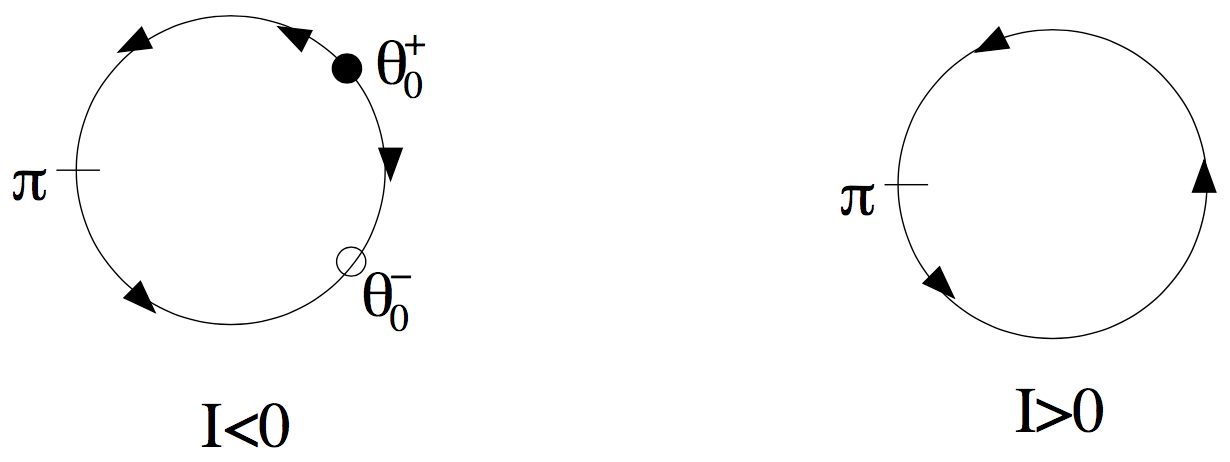
\includegraphics[width=0.6\columnwidth]{phase_circle}
\caption{
\textbf{Phase circle of the theta model.}
The neuron fires every time $\theta$ crosses $\pi$.
For $I < 0$ there are two fixed points: An unstable point $\theta_0^+ = \arccos\frac{1 + \alpha I}{1-\alpha I}$,
and an attractor (stable point) $\theta_0^- = -\theta_0^+$.}
\label{phase_circle}
\end{figure}

\subsection{Synaptic Interactions}

The input current $I$ is the sum of a constant current $I_0$ and transient synaptic currents $I_i(t)$, 
where $i \in 1..N$ indexes the synapses:
\begin{equation}
	I = I_0 + \sum_{i=1}^N I_i(t)
\end{equation}
Synaptic currents are modeled as Diracs: $I_i(t) = w_i\delta(t - t_i)$,
where $t_i$ is the firing time of presynaptic neuron $i$ and $w_i$ the weight of the synapse.

One tricky problem is the calculation of the Dirac delta function $\delta$. 
The author did not mention in the paper how he compute the $\delta(t-t_i)$.
By definition we know % \equation{}
\begin{equation}
\label{dirac}
\delta(t-t_i) = \left\{ \begin{array}{ll}
 A & \textrm{if $t = t_i$}\\
 0 & \textrm{otherwise}
  \end{array} \right.
\end{equation}
but we don't know the choice of $A$.
We were too young too simple and took $1.0$ for $A$, which resulted in mismatch between
the experiment results obtained by us and the author. 
After long time of debugging we find that a larger $A$ is necessary for reproducing the experiment result shown in
the paper.

\subsection{Response Property Analysis of the Theta Model}

We successfully reproduce the simulation results of the relation of the firing time of a theta neuron and the time of arrival of a synaptic current, as shown in Figure~\ref{response}. The results are precisely similar to that shown in the paper.


\begin{figure}
\centering
\subfigure[$I_0 > 0$]{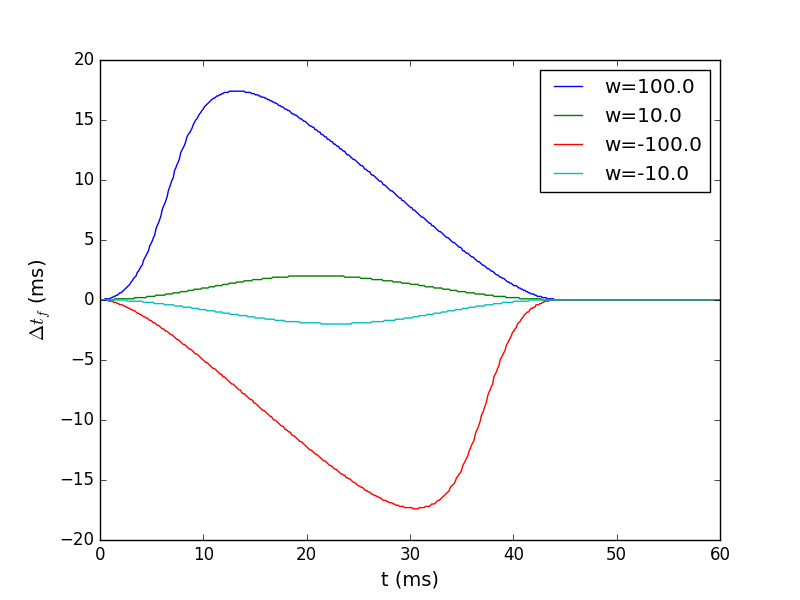
\includegraphics[width=0.98\columnwidth]{response_pos}}
\subfigure[$I_0 < 0$]{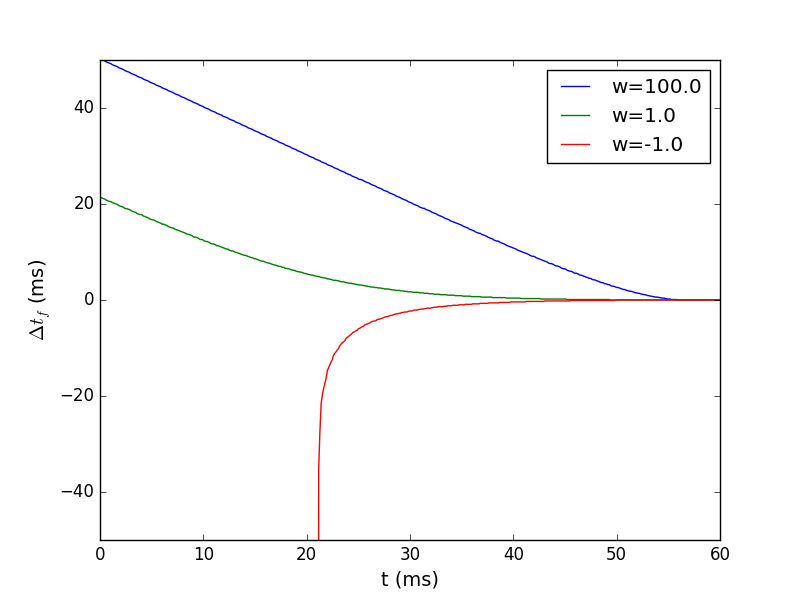
\includegraphics[width=0.98\columnwidth]{response_minus}}
\caption{\textbf{Response properties of the theta model.}
(a) For $I_0 > 0$, the neuron spikes regularly ($I_0 = 0.005$, $\theta(0) = -\pi$). 
The positive curve is called the \emph{Phase Response Curve} (PRC).
(b) Response for $I_0 < 0$.
The initial condition is slightly above the unstable equilibrium point $(I_0 = -0.005, \theta_0 = \theta_0^+ + 0.0001)$.}
\label{response}
\end{figure}

In the time coding model, we view this curve as the transfer function of the neuron; 
it describes how the neuron converts input spike times into output spike times.
Specifically, the curve describes how long the neuron theta will fire \emph{in advance}
(with respect to the firing time without any input presynaptic current) 
when it receives a Dirac current of weight $w$ at time $t$. 


\begin{figure}
\centering
\subfigure[$I_0 > 0$]{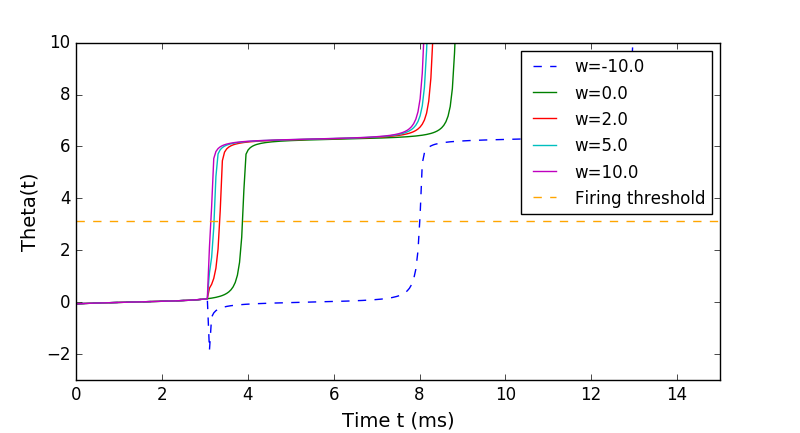
\includegraphics[width=0.98\columnwidth]{theta_t_positive_I}}
\subfigure[$I_0 < 0$]{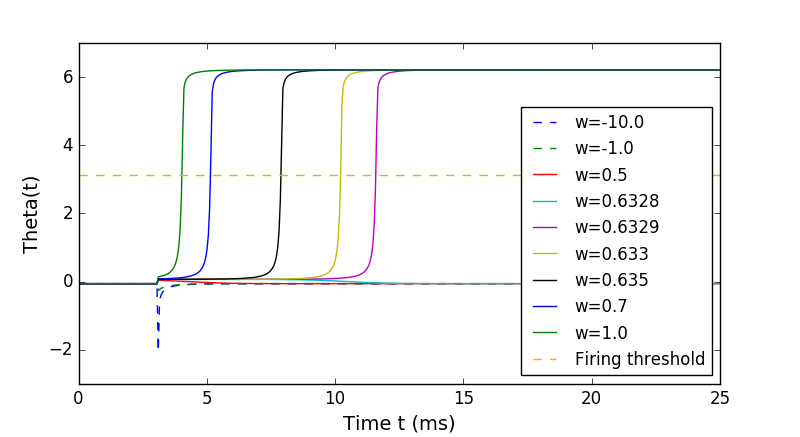
\includegraphics[width=0.98\columnwidth]{theta_t_negtive_I}}
\caption{The relation between $\theta$ and $t$ given different values of $w$. 
There is only one single presynaptic neuron whose firing time is $t_i = 3.0$ ms.
(a) $I_0 = +0.01$. (b) $I_0 = -0.01$. ($\theta_0 = \theta_0^-$ and $\alpha = 0.1$ in both subfigures.)}
\label{theta_t}
\end{figure}

Let's take a closer look at the response properties shown in Figure~\ref{response}.
When $I_0 > 0$, we have seen before that the theta neuron always fires, and from the figure 
we can see that whether it fires earlier or later depends on the sign of the current weight $w$. 
Assume $w$ is positive, we can see that $\Delta t_f$ equals to or is close to $0$ both when $t$ is
small enough and large enough, and $\Delta t_f$ reaches its maximum when $t$ takes a median value.
The reason is two-folded.
On one hand, when $t$ is very small, the input Dirac current comes when $\theta$ is close to the initial
value $\theta(0) = -\pi$, thus $1+\cos \theta$ is close to $0$, and the Dirac current $I$ hardly has any
impact on $\frac {d \theta}{dt}$, let alone impact on $\theta$.
On the other hand, when $t$ is large, the $\theta$ has already been near
to the firing threshold, and the marginal revenue of receiving an input Dirac current at that time is small.
When $t$ is sufficiently large (larger than the firing cycle), the theta neuron fires before the arrival
of the input Dirac current, and thus the firing time is not affected by $t$ anymore.

When $I_0 < 0$, things are more interesting. When $w > 0$, the $\Delta t_f$ is monotone decreasing
with $t$, indicating that the input Dirac current has larger impact when it comes earlier.
When $t$ is sufficiently large and the theta neuron fires first, 
$\Delta t_f$ becomes $0$ for the same reason described above.
However, when $w < 0$ and $t$ is small enough, the theta neuron no longer fires. This is because
when $\theta$ is not too far from the initial value $\theta_0^+$, the input Dirac current, which decreases
$\theta$ when $w < 0$, may take $\theta$ into the range $(-\pi, \theta_0^+)$, ending up with
$\theta = \theta_0^-$. That's why in Figure~\ref{response}(b) the $\Delta t_f$ is unbounded when $t$ is small.


We further show the change of $\theta$ over time by simulations.
We set the arrival time $t$ of the input Dirac current to $3.0$ ms in all simulations.
The results are shown in Figure~\ref{theta_t}.
From Figure~\ref{theta_t}(a) we can see that the theta neuron always fires no matter what the sign
of $w$ is. Positive $w$ makes the theta neuron fires earlier, and vice versa. 
From Figure~\ref{theta_t}(b) we can see that the theta neuron fires when $w=0.6329$, while it never
fires when $w \leq 0.6328$, which means the behavior of the neuron could be very sensitive to the value of
the synapse weight $w$ under certain circumstances.


\subsection{Learning Rule}

The derivation of the learning rule is detailed and clear in the paper. 
We do not repeat the derivation process in this report but highlight some key ideas of it.

Our objective is to learn a set of target firing times $\bar t_s$. That is, we train a set of theta neurons
to fire at the time we would like them to fire. The loss function (cost function) is the mean square error,
denoted by $E = \langle t_s - \bar {t}_s$, where $t_s$ are the actual spike times.
The original work use gradient descent method to optimize $E$, so the derivation of the learning rule
is just computations of partial derivatives.

The firing time $t_s$ is not directly a function of $w_i$, so the author defined a function $F$ 
(see Equation~\ref{F_t}) 
denoting the ``\emph{remaining time}'', i.e., the time that remains before the theta neuron will fire, and thus turned
the calculation of $\frac{\partial t_s}{\partial w_i}$ into calculation of $\frac{\partial F(t)}{\partial w_i}$
($t$ is the current time). 

\begin{equation}
\label{F_t}
	F(t) = \int_{\theta(t)}^\pi \frac{d \theta}{(1-\cos \theta) + \alpha I (1 + \cos \theta)}
\end{equation}

The problem is that $I$ is not continuous, making it unpractical to directly compute $\frac{\partial F(t)}{\partial w_i}$. 
The discontinuity comes from the occurrences of multiple input Dirac currents,
making $I$ and further the integrand a piecewise continuous function.
So the key idea is to break the time domain at $t_i$s ($t_i$ is the time of the $i$-th input Dirac current), 
and compute the derivatives on the intervals.

The final learning rule is described by the following equation:
\begin{equation}
\Delta w_i =
\left\{ \begin{array}{lr}
 -2\eta (t_s - \bar{t}_s) \frac{\partial t_s}{\partial w_i} & \text{if } 0 < - \frac{\partial t_s}{\partial w_i}  < C\\
2\eta (t_s - \bar{t}_s) C & \text{otherwise}
  \end{array} \right.
\end{equation}






\section{Auto-encoder Network Evaluation}
\label{exp}

In this section, we firstly briefly review the auto-encoder network model constructed with theta neurons
proposed in the paper, and then describe how we reproduce the results of the experiments conducted by the author.

\begin{figure}
\centering
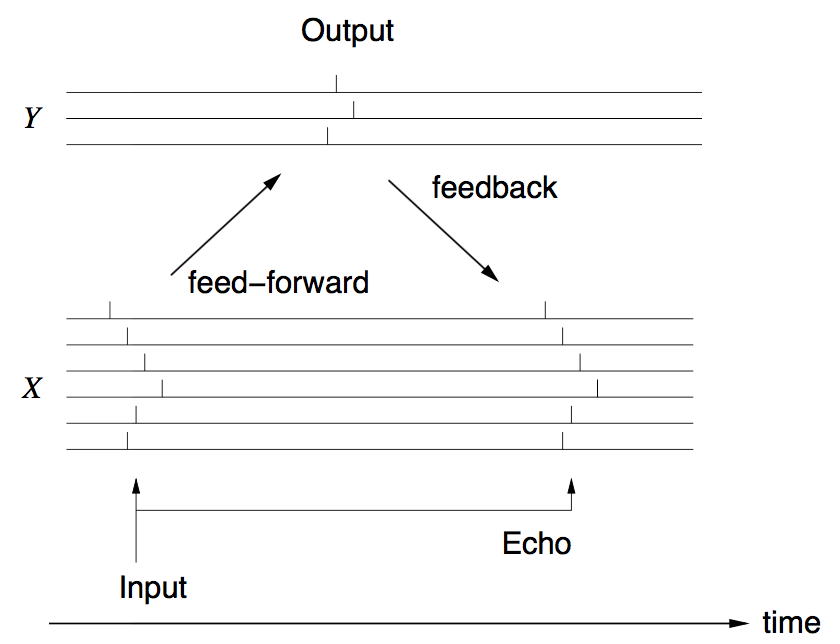
\includegraphics[width=0.98\columnwidth]{network}
\caption{The auto-encoder network tries to reconstruct the input spikes at target firing times (the echo of the input burst).
}
\label{auto_encoder}
\end{figure}

In the original paper, the author explains how to train a network to predict its own activities using the learning rule derived above. 
The prediction objective is a time-delayed version of the input (echo), 
and the network has to find a representation of the input that minimizes mean squared reconstruction error.
Figure~\ref{auto_encoder} shows the simplified architecture of the auto-encoder network.
The network consists of three layers of neurons: 
an input population $X$ of size $n$ neurons represents the input vectors using spike times; 
an output population $Y$ of size $m$ neurons is activated by neurons in $X$; 
a reconstruction population $X'$ of size $n$ neurons is activated by neurons in $Y$ and reconstructs the input (with a predefined delay).

Usually $m < n$, so what the auto-encoder network does is to learn a compact representation of the input data,
and reconstruct the input from the representation. 
We can also view the process as reducing the dimension (compressing) of the original input data,
and then reconstructing them.
We hope to find a good representation so that the reconstruction error (the difference between the reconstructed
data and the original data) is as little as possible.

The author proposes in the paper that if the spike times are within the linear part of the response curve,
then the auto-encoder network performs Principal Component Analysis (PCA) in the time domain.
And in the experiment section of the paper, the author shows how to train an auto-encoder network to compute PCA
of a two-dimensional Gaussian distribution.
We redid all the experiments mentioned in the paper. 
In the following subsection, 
we describe our experiment results and focus on comparing the results obtained by the author and us.

\subsection{PCA of a Gaussian Distribution}

In this experiment, we use three input neurons to encode a two-dimensional Gaussian random variable.
Specifically, the spike times of the three neurons (denoted by $t_0$, $t_1$, and $t_2$) encode the two 
dimensions of the Gaussian random variable by the two relative spike times $t_1 - t_0$ and $t_2 - t_0$, 
where the spike time of the first neuron $t_0$ is used as an absolute time reference.

We construct the 3-2-3 network ($n=3$, $m=2$) and set the parameters such as $ISI$ and $C$ to the same
value described in the paper.
We randomly generate 500 input sample points and use them to train the auto-encoder network.
The evolution of the six weights over iterations are shown in Figure~\ref{local_minimum}.
We can see that the weight converges to a stable solution, and the MSE significantly decreases.
However, the learned weight matrix is only a local optimal solution, as the reconstructed $t_i$s for each input sample
always satisfy that $t_0 \approx t_1 \approx t_2$. 
That's why in Figure~\ref{local_minimum}(c) we see that the reconstructed relative spike time is always $0$,
no matter what the $\bar t_i$s (the desired spike times) are.
Note that the author didn't mention the problem of local minimum, 
neither did he explain why in Figure 5 of the original paper, the weights converge to a value near
1.5 in the beginning but diverge after several hundred of iterations even though the learning rate $\eta$
is only 0.0001 as provided in the paper.

To get out of the local minimum, we have to increase the learning rate $\eta$. 
Practically, we change $\eta$ to nearly $0.1$ and continue training starting from the weights of 
the local minimum solution. The results are shown in Figure~\ref{local_better}.
We can see that the weights diverge at first, and then become stable or oscillate around some fixed values,
and the MSE decreases to a lower level.

However, the weight matrix is still local optimal, 
as we can see in Figure~\ref{local_better} the reconstruction error of points
satisfying $t_1 < t_0$ and $t_2 < t_0$ (``negative samples'') is relatively large. 
In other words, the auto-encoder network successfully learns one direction of the principal component but fails
to learn the other one. To solve the problem, we dynamically set a higher learning rate $\eta$ when
the model is fed with samples where $t_1 < t_0$ and $t_2 < t_0$ and a lower learning rate otherwise,
which is equivalent to resampling the negative samples.
In this way, we get results shown in Figure~\ref{global_best}.
Some of the weights oscillate again, and then all weights become stable (see Figure~\ref{global_best}(a)).
The MSE further decreases (see Figure~\ref{global_best}(b)).
The shape of the reconstructed principal directions is exactly the same with that shown in the paper.
We finally reproduce the PCA results successfully.

The reason why the author could train the model to do PCA without dynamically tuning the learning rate is not yet known.
All experiments we conducted using the exactly same parameters as the author showed in the paper failed to reconstruct the principal directions as the weight matrix always ended up in a local optimal solution.
We discuss this mismatch more in Section~\ref{discussion}.

\begin{figure*}
\centering
\subfigure[$w_i$s]{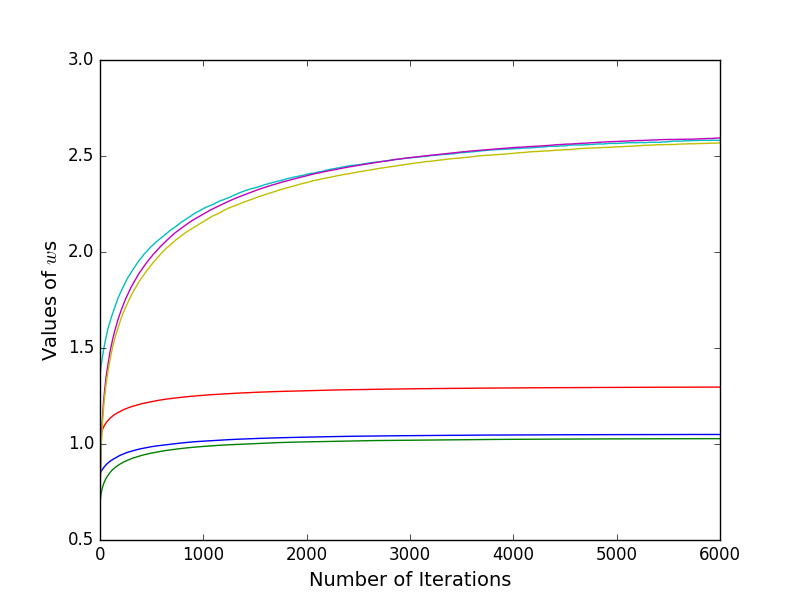
\includegraphics[width=0.68\columnwidth]{local_min_weight_evolution}}
\subfigure[MSE]{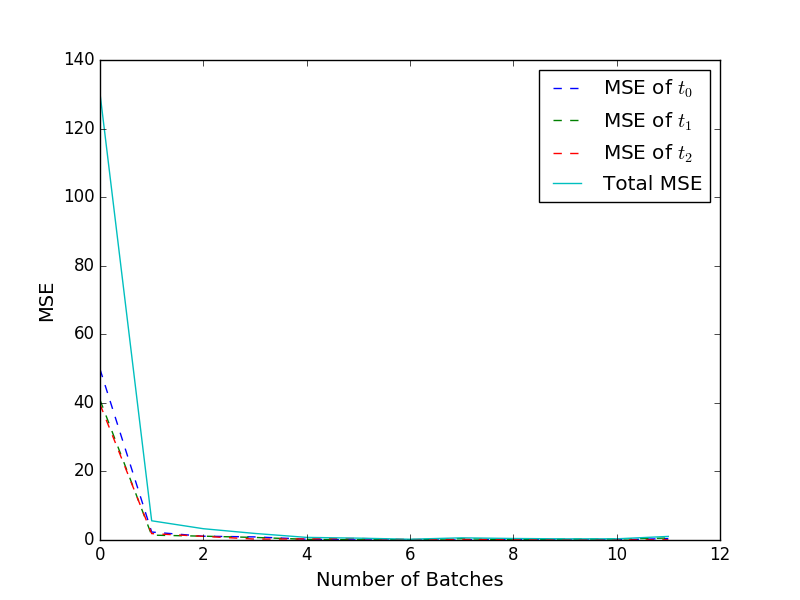
\includegraphics[width=0.68\columnwidth]{local_min_mse}}
\subfigure[Reconstructed $t_i$s]{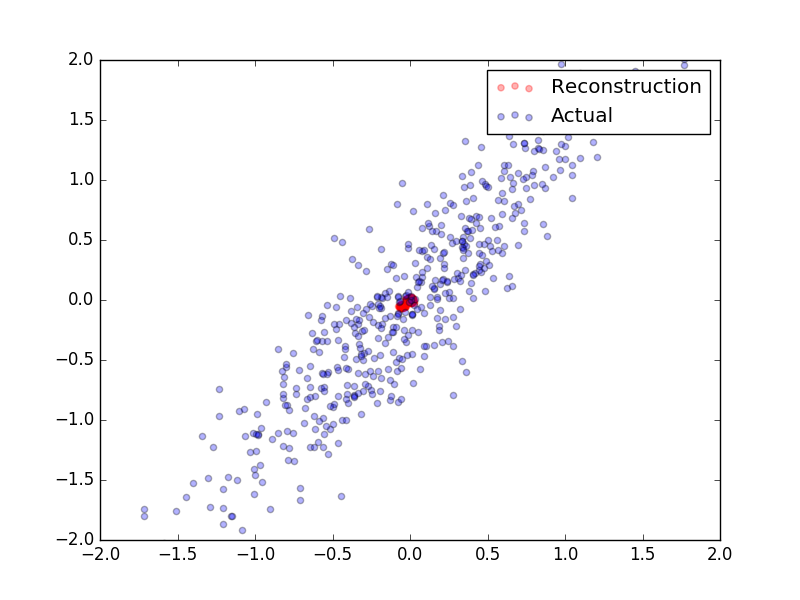
\includegraphics[width=0.68\columnwidth]{local_min_t}}
\caption{The MSE coverages but the weight matrix is trapped into a local minimum point and fails to come out.
(a): The evolution of the weights over iterations.
(b): The evolution of the mean square errors over iterations.
(c): The reconstructed $t_1-t_0$ and $t_2-t_0$.}
\label{local_minimum}
\end{figure*}

\begin{figure*}
\centering
\subfigure[$w_i$s]{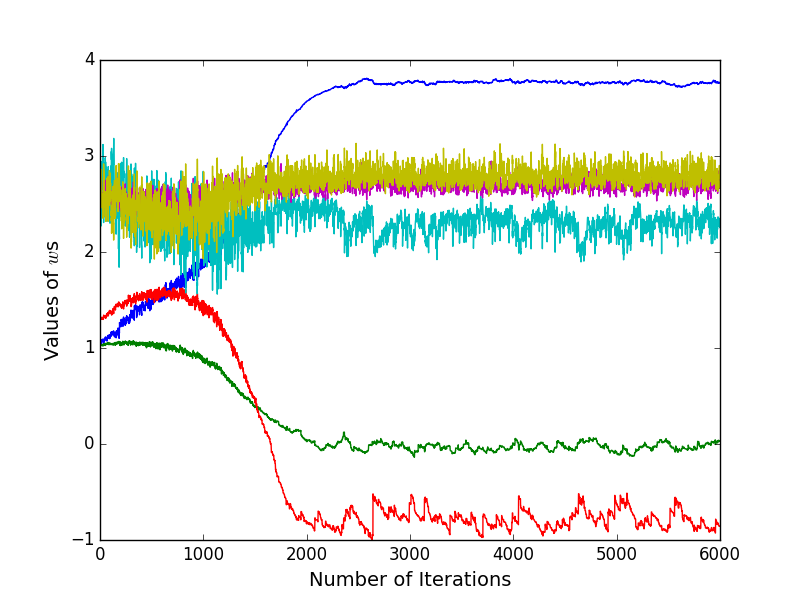
\includegraphics[width=0.68\columnwidth]{local_better_weight_evolution}}
\subfigure[MSE]{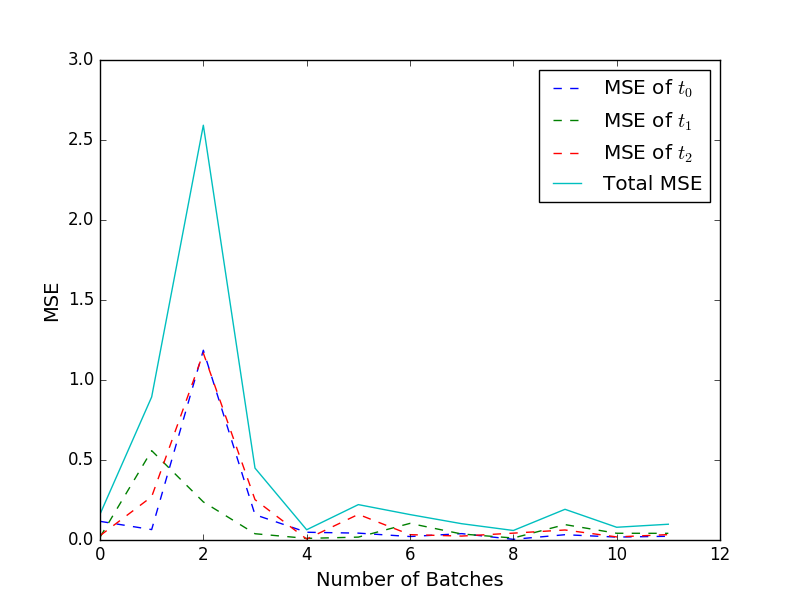
\includegraphics[width=0.68\columnwidth]{local_better_mse}}
\subfigure[Reconstructed $t_i$s]{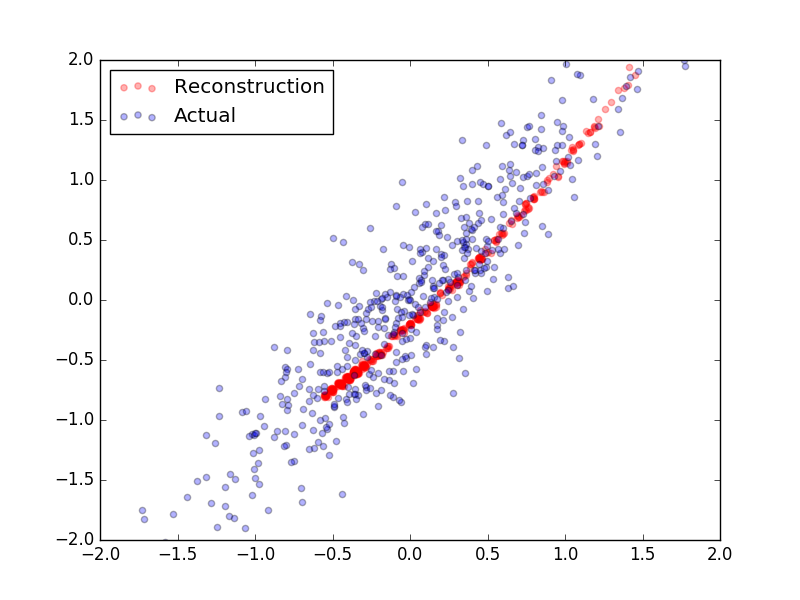
\includegraphics[width=0.68\columnwidth]{local_better_t}}
\caption{The weight matrix gets out of the local minimum point and converges to a better solution,
but it is trapped into another local minimum as
the reconstruction error is relatively large when $t_1 < t_0$ and $t_2 < t_0$.
(a): The evolution of the weights over iterations.
(b): The evolution of the mean square errors over iterations.
(c): The reconstructed $t_1-t_0$ and $t_2-t_0$.}
\label{local_better}
\end{figure*}

\begin{figure*}
\centering
\subfigure[$w_i$s]{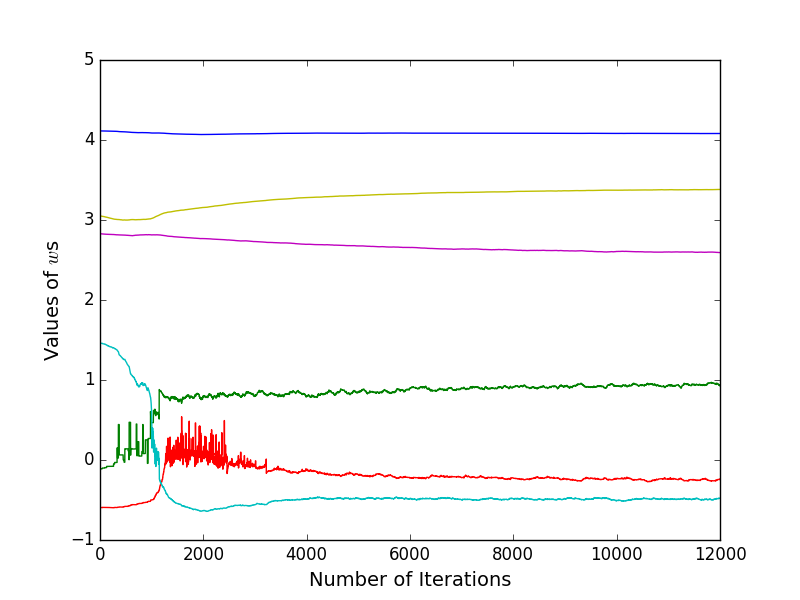
\includegraphics[width=0.68\columnwidth]{global_weight_evolution}}
\subfigure[MSE]{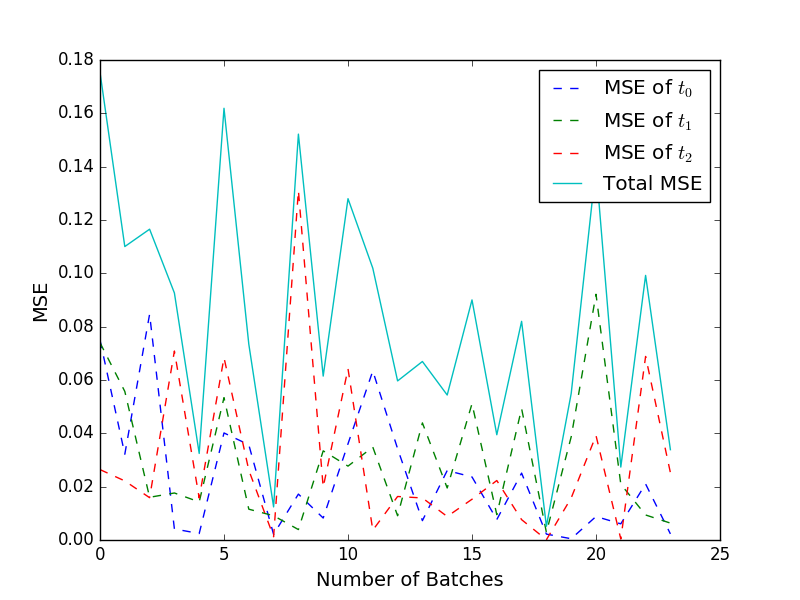
\includegraphics[width=0.68\columnwidth]{global_mse}}
\subfigure[Reconstructed $t_i$s]{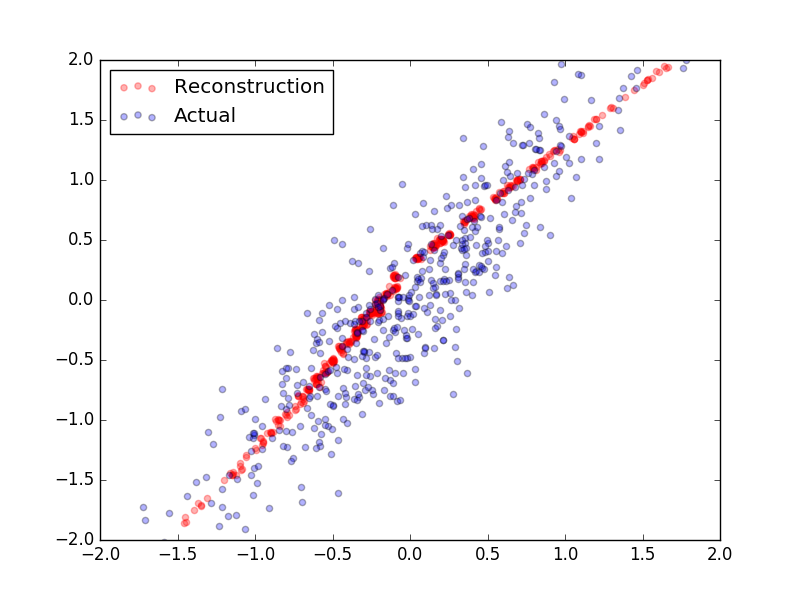
\includegraphics[width=0.68\columnwidth]{longer_better_t}}
\caption{Again the weight matrix gets out of the local minimum point and converges,
the total MSE further decreases, and the principal components are well reconstructed.
(a): The evolution of the weights over iterations.
(b): The evolution of the mean square errors over iterations.
(c): The reconstructed $t_1-t_0$ and $t_2-t_0$.}
\label{global_best}
\end{figure*}

\subsection{Encoding Natural Images}
Similarly, we continue working on the natural image encoding experiment mentioned in the paper. We use the same image dataset as the author's, which contains 10 gray images of size $512 \times 512$. We are supposed to randomly draw $16 \times 16$ patches from the gray images as our network input, normalizing all samples to scale their standard variation to 1. The encoder network has an architecture of $256\times 64 \times 256$, which means, the number of weight parameters to be trained in this network is over 10,000. Usually, we need a larger number of samples than weights to train a network model, however, with constraints of computation capacity, we only pick one $512 \times 512$ image, divide it to 1024 patches as the training data. To verify the correctness of the model, we reconstruct the same image with trained weights, to see whether a sparsely represented image could be obtained.

Unfortunately, we found tuning of parameters in this experiment is even harder than PCA. We adopt all parameters mentioned in paper, and adjust amplitude gain of Dirac current to be a reasonable value. Normalized to have a standard deviation of 1, the input value ranges from 0 to 4.8, which is a large range comparing to PCA case. The actual firing time can hardly fit the desired firing time, with weights updated every step by various samples.

We have tried different scales of learning rate $\eta$, as well as other parameters such like $C$, and $\lambda$. None of our trails results in a consistent convergence of MSE. We quite doubt on how the author tuned the parameter in such a non-convex problem, and how he avoid being trapped into local minima.



\section{Discussion}
\label{discussion}

The auto-encoder network model is extremely sensitive to the parameters.
This sensitivity makes the model very hard to tune and to train when the number of the parameters grows.
The author gave the heuristic choices of the parameters for his experiments in the paper, 
but he did not give any insight about how to choose them. 
The model won't work (converge during training) unless the parameters such as 
$\alpha$, $\lambda$ and $I_0$ are carefully chosen.
Moreover, the author did not either mention how he calculated the delta dirac function 
(we don't know the value of $A$ in Equation~\ref{dirac} i.e. the amplitude of the input
dirac current. We try some values but only a few work).
Practically, we find that the given parameters partially works in the 2-D gaussian distribution experiment, 
while they do not work in the natural image experiment,
as the training process is either unstable or trapped into a local minimum. 
Therefore we don't believe the method and the auto-encoder network architecture is practical and generalize well
as long as it is sensitive to the parameters, which have to be heuristically chosen by human.

Another limitation of the proposed auto-encoder model is that it only works with specific cases
(using theta neurons to compute PCA).
The method only works with a single-layer of neurons, and cannot approximate complex functions.
Also, it made certain assumptions about the gradient derivation, which makes training unpractical in some other cases.

Some subsequent research such as~\cite{mckennoch2009spike} partially solved the problems mentioned above,
designed more advanced learning rule, 
and generalized the theta neuron network to solve more sophisticated machine learning tasks such as regression and classification.
Despite that the problem of parameter sensitivity still existed as the authors spent a whole page 
discussing parameter sensitivity, the work still showed the great potential of temporal-coding and time-based computation.


\section{Errors in the Paper}
\label{error}

In this section we list some suspected errors in the paper.

\paragraph{Error 1.}
In Equation (6) of page 3 of the paper, the potential after the synaptic current are computed as
\begin{equation}
	\theta_j^+ = \theta(t_j^+) = \theta_j^- + \alpha w_j (1+\cos \theta_j^-)
\end{equation}
Firstly, we think it should be 
\begin{equation}
	\theta_j^+ = \theta(t_j^+) = \theta_j^- + (1-\cos \theta_j^-) + \alpha w_j (1+\cos \theta_j^-)
\end{equation}
We see no reason why the term $ 1-\cos \theta_j^-$ is removed.
Secondly, this equation is very misleading because it does not explicitly show the length of timestep $dt$,
or it just takes $1.0$ for the timestep.
Precisely, we should use the following formula to update $\theta$:
\begin{align}
	\theta_j^+ &= \theta(t_j^+) \\
	&= \theta_j^- + d\theta \\
	&= \theta_j^- + \frac{d\theta}{dt} dt\\
	&= \theta_j^- + ((1-\cos \theta_j^-) + \alpha w_j (1+\cos \theta_j^-))dt
\end{align}
where $dt$ is not necessarily $1.0$, which is very import for the implementation.


\paragraph{Error 2.} 
In Equation (11) of page 4 of the paper, one condition brach is
\begin{equation}
	\textrm{if } 0 < -\frac{\partial t_s}{\partial w_i} < C,
	\textrm{ then: } \Delta w_i = -2\eta(t_s - \bar{t_s}) \frac{\partial t_s}{\partial w_i}
\end{equation}
We think the condition should be $\textrm{if } 0 \leq -\frac{\partial t_s}{\partial w_i} < C$.
Intuitively, if we have reached the global optimal point, where $\frac{\partial t_s}{\partial w_i} = 0$ for all $w_i$s,
we should be happy with the current weight matrix
instead of adding a large bias ($\eta(t_s - \bar{t_s}) C$) to the weights $w_i$s.
The first ``$<$'' in the condition makes the gradient descent algorithm unstable near the optimal points.

\paragraph{Error 3.} 
In the second paragraph of Section 3 of the paper, the author wrote:
``The learning rule updates the feedback connections $(w_{ij})_{i\leq n,j\leq m}$ from $Y$ to $X$...''
Obviously there is a typo. It should be ``from $Y$ to $X'$'' instead of ``from $Y$ to $X$''.

\paragraph{Error 4.}
There is a small typo in the last paragraph of Section 2.3. 
It should be ``to the case $\theta_i^+ \in [\theta_0^-, \theta_0^+]$'' instead of 
``to the case $\theta_i^+ \in [\theta_0^-\theta_0^+[$''.






{\small
\bibliographystyle{ieee}
\bibliography{ref}
}

\end{document}
